\chapter{数列、数学归纳法、数列的极限}

\section*{一、数列的一般概念}
\section{数列的定义}

\noindent
\begin{minipage}{.5\textwidth}
    \CTEXindent
我们看下面的例子:

图5.1表示堆放的钢管,
共堆放了7层,自上而下各层
的钢管数排列成一列数:
\[4,\quad 5,\quad 6,\quad 7,\quad 8,\quad 9,\quad 10\]

自然数$1,2,3,4,5,\ldots$的倒数排列成一列数:
\[1,\quad \frac{1}{2},\quad \frac{1}{3},\quad \frac{1}{4},\quad \frac{1}{5},\quad\ldots\]
\end{minipage}\hfill
\begin{minipage}{.4\textwidth}
    \centering
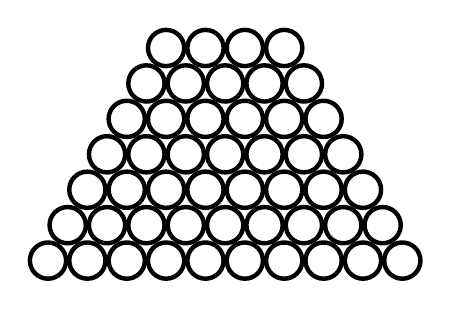
\begin{tikzpicture}
  \foreach \x in {1,2,3,...,10}
{
    \draw[ultra thick](\x/2,0)circle(.23);
}  
\foreach \x in {1,2,3,...,9}
{
    \draw[ultra thick](\x/2+.25,.45)circle(.23);
}  
\foreach \x in {1,2,3,...,8}
{
    \draw[ultra thick](\x/2+.5,.9)circle(.23);
}  
\foreach \x in {1,2,3,...,7}
{
    \draw[ultra thick](\x/2+.75,.45*3)circle(.23);
}  
\foreach \x in {1,2,3,...,6}
{
    \draw[ultra thick](\x/2+1,.9*2)circle(.23);
}  
\foreach \x in {1,2,3,...,5}
{
    \draw[ultra thick](\x/2+1.25,.45*5)circle(.23);
}  
\foreach \x in {1,2,3,4}
{
    \draw[ultra thick](\x/2+1.5,.9*3)circle(.23);
}  



\end{tikzpicture}
\captionof{figure}{ }

\end{minipage}

$\sqrt{2}$的精确到$1, 0.1, 0.01, 0.001,\ldots$的不足近似值
排列成一列数:
\[1,\quad 1.4,\quad 1.41,\quad 1.414,\quad \ldots\]    

$-1$的1次幂,2次幂,3次幂,4次幂,……排列成一列
数:
\[-1,\quad 1,\quad -1,\quad 1, \quad\ldots\]

再看下面的例子:

函数$y=\frac{1}{x^{3}}$, 当$x$依次取$1,2,3,\ldots,n\; (n\in\N)$时,得到一列数:
\[1, \frac 18, \frac {1}{27}, \ldots, \frac {1}{m^{3}}\]

函数$y=x^{2}-1$, 当$x$依次取$1,2,3,4,\ldots,n\; (n\in \N)$
时,得到一列数
$$0,\; 3,\; 8,\; 15,\ldots,\; n^{2}-1$$

象上面这些例子,按一定顺序排列的一列数叫做\textbf{数列}。数列中的每一个数都叫做这个数列的\textbf{项},各项依次叫做这个数列的第1项(或首项),第2项,第3项,……,第$n$项.

在一个数列中,它的任一项的数值,由它所对应的项数唯一确定,因此数列中各项的值是其项数的 函数,即$a_n=f(n)$, 其中$a_n$表示第$n$项。$n$为自变量$(n\in\mathbb{N})$, 第$n$项为$a_n$的数列记作$\{a_n\}$.

\section{数列的表示法}
数列实质上就是其定义域是自然数集$\N$(或$\N$的有限子
集$\{1,2,\ldots,n\}$)的函数,因此数列的表示方法与过去所学
的函数的表示方法完全类似。

\subsection{列表法表示数列}
将数列的各项依次列举出来:
\[a_1,a_2,a_3,a_4,\ldots, a_n, \ldots\]
其中$a_n$
表示数列第$n$项的数值,$n$是它的项数。显然$a_n$是$n$的函
数。

\subsection{图象法表示数列}

\begin{figure}[htp]
    \centering
\begin{tikzpicture}[>=stealth, scale=.5]
\begin{scope}
\draw[->](-1,0)--(7,0)node[below]{$n$};
\draw[->](0,-3)--(0,8)node[left]{$a_n$};
\foreach \x/\y in {3/1,4/3,5/5,6/7}
{
    \draw[dashed](0,\y)node[left]{$\y$}--(\x, \y)--(\x,0)node[below]{$\x$};
}
\foreach \x/\y in {1/-2,2/-1}
{
    \draw[dashed](0,\y)node[left]{$\y$}--(\x, \y)--(\x,0)node[above]{$\x$};
}
\node[below left]{$O$};
\node at (4,-2){(1)};
\end{scope}
\begin{scope}[xshift=12cm]
    \draw[->](-1,0)--(7,0)node[below]{$n$};
\draw[->](0,-1)--(0,7)node[left]{$a_n$};
\foreach \x in {1,2,3,4,5,6}
{
    \draw[dashed](\x,0)node[below]{$\x$}--(\x,{5-5/(\x+1)})--(0,{5-5/(\x+1)});
}
\node[below left]{$O$};
\node at (3,-2){(2)};
\node at (0,2.5)[left]{$\tfrac{1}{2}$};
\node at (0,4.16)[left]{$\tfrac{5}{6}$};
\draw(0,5)node[left]{1}--(.1,5);

\end{scope}
\end{tikzpicture}
    \caption{}
\end{figure}

图5.2(1)表示数列$-3,-1,1,3,5,7,\ldots$; 图5.2(2)表示数列
$\frac{1}{2},\frac{2}{3},\frac{3}{4},\frac{4}{5},\frac{5}{6},\ldots$.

用图象法表示数列时,图象是由直角坐标系中的一些孤
立点组成,其中每一个点$(n,a_n)$
的横坐标$n$表示项数,纵坐标$a_n$表示该项的值,用图象表示数列时,其两个坐标轴上的单位可以不同。

\subsection{解析法表示数列}
如果数列的第$n$项$a_n$能用项数$n$的解析式表示为:
$a_n=f(n)\; (n\in\N)$。这种表示方法称为解析法,这个解析式叫做数列的\textbf{通项公式}。

图5.2(1)所表示的数列的通项公式
$a_n=2n-5$; 图
5.2(2)所表示的数列的通项公式为$a_n=\frac{n}{n+1}$.

不是所有的数列都能用解析法来表示。例如$\sqrt{2}$
的精
确到$1,0.1,0.01,0.001,\ldots$的不足近似值组成的数列$1,
1.4,1.41,1.414,\ldots$就没有通项公式。

\subsection{用递推式表示数列}
有时数列可以用它的前几项的值(称初始条件或初始
值),和数列中相邻若干项间的关系式(称递推式)给出。例
如一个数列$\{a_n\}$
中,
$a_1=1$,
$a_{n+1}=2a_{n}+1\; (n\in\N)$
,这个数列
就是$1,3,7,15,31,63,\ldots$; 又如数列$2,5,8,11,14,
\ldots$, 可以表示为:
$a_1=2$, $a_{n+1}=a_n+3$.

\begin{ex}
    按照下列条件,写出数列的前五项。
\begin{enumerate}
    \item 数列的通项公式是:
\begin{multicols}{2}
\begin{enumerate}[(1)]
    \item $a_n=-3n+1$
    \item $a_n=\left(\frac{1}{2}\right)^n$
    \item $a_n=\frac{2n-1}{n+1}$
    \item $a_n=n^2+2$
\end{enumerate}    
\end{multicols}
\item 数列$\{a_n\}$中,已知
$a_1=2$,且$(n\in\N)$.
\item 数列$\{a_n\}$的图象如图5.3.
\end{enumerate}
\end{ex}

\begin{center}
\begin{tikzpicture}[>=stealth, scale=.6]
 \draw[->](-1,0)--(7,0)node[below]{$n$};
\draw[->](0,-3)--(0,4)node[right]{$a_n$};
\foreach \x in {1,2,3,4,5,6}
{
   \draw(\x,0)node[below]{$\x$}--(\x,.1);
}
\foreach \x in {1,2,3,-1,-2}
{
   \draw(0,\x)node[left]{$\x$}--(.1,\x);
}
\draw[dashed](0,-2)--(3,-2)--(3,0);
\draw[dashed](0,-1)--(5,-1)--(5,0);
\draw[dashed](0,.5)node[left]{$\tfrac{1}{2}$}--(6,.5)--(6,0);
\draw[dashed](0,3)--(2,3)--(2,0);
\draw[dashed](0,1)--(4,1)--(4,0);
\node[below left]{$O$};
\end{tikzpicture}
\captionof{figure}{ }
\end{center}

\section{简单数列的通项公式的求法}
用语言叙述或用列表法给出的一些数列的前几项,我们
可以利用归纳的办法,写出它们的通项公式。

\begin{example}
    写出下列各数列的通项公式。
\begin{enumerate}[(1)]
\item 自然数的倒数组成的数列;
\item 每项的值都比项数的立方少2的数列;
\item $-1$的自然数次幂组成的数列。
\end{enumerate}
\end{example}

\begin{solution}
\begin{multicols}{3}
  \begin{enumerate}[(1)]
    \item $a_n=\frac{1}{n}$
    \item $a_n=n^3-2$
    \item $a_n=(-1)^n$
\end{enumerate}  
\end{multicols}
\end{solution}

\begin{example}
    写出下列各数列的一个通项公式,使其前六项分
别是:
\begin{enumerate}[(1)]
\item  $\frac 12,\; \frac 34, \;\frac 78,\; \frac {15}{16} , \; \frac {31}{32} , \; \frac {63}{64}$
\item $2,\; -6,\; 18,\; -54,\; 162,\; -486$
\item $-1,\; \frac{3}{2},\; -\frac{1}{3},\; \frac{3}{4},\; -\frac{1}{5},\; \frac{3}{6}$
\item $9,\; 99,\; 999,\; 9999,\; 99999,\; 999999$
\end{enumerate}

\end{example}

\begin{solution}
\begin{enumerate}[(1)]
    \item 分母为$2^n$,分子均比分母少1, 所以数列的通
    项公式为$a_n=\frac{2^n-1}{2^n}$
    \item 分析数列的前6项发现,第1项是2, 第2项是
    2的$-3$倍,第3项又是第二项的$-3$倍,以此类推,可归纳
    出其通项公式为
    $a_n=2\x(-3)^{n-1}$
    \item 数列各项的分母依次为$1,2,\ldots$, 恰与项数相同;
    各项的分子为$1,3,1,3,\ldots$, 可以说是第1项比2少1,
    第2项比2多1, 以此类推;又数列相邻两项值的符号相
    反,且第1项为负值,因此可用符号$(-1)^n$来表示,由此归
    纳可得通项公式为
    $a_n=(-1)^{n}\frac{2+(-1)^n}{n}$.
    \item 数列第1项可改写为$10-1$, 第2项为
    $10^2-1$,……
    故通项公式为$a_n=10^n-1$.
\end{enumerate}
\end{solution}

\begin{rmk}
\begin{enumerate}[(1)]
    \item  分析数列中各项的值与项数间的关系,从而
    归纳出通项公式,是求数列通项公式的最基本的方法。
    \item 给出数列的前几项,求这个数列的通项公式时,
    其通项公式并不是唯一的。事实上,满足一个数列的前若干
    项的通项公式可以有无穷多个。例如,上例中的(1)的通
    项公式可以写成:
\[a_n=\frac{2^n-1}{2^n}+(n-1)(n-2)(n-3)(n-4)(n-5)(n-6)\cdot f(n)\]
(其中$f(n)$
是含$n$的任何一个函数式),其前六项均符合要
求,这是因为公式的后一部分,当$n$依次取$1,2,3,4,5,
6$时,其值都是0.
\end{enumerate}
\end{rmk}

\begin{ex}
\begin{enumerate}
    \item 写出数列的一个通项公式,使得数列的前五项分别是
\begin{enumerate}[(1)]
    \item $15,\; 25,\; 35,\; 45,\; 55$
    \item $1,\; -\frac{1}{2},\; \frac{1}{4},\; -\frac{1}{8},\; \frac{1}{16}$
    \item $1,\; 3,\; 5,\; 7,\; 9$
    \item $1-\frac{1}{2},\; \frac{1}{2}-\frac{1}{3},\; \frac{1}{3}-\frac{1}{4},\; \frac{1}{4}-\frac{1}{5},\; \frac{1}{5}-\frac{1}{6}$
    \item $0,\; -5,\; 8,\; -17,\; 24$
    \item $3,\; 33,\; 333,\; 3333,\; 33333$
\end{enumerate}
\item 观察下列数列的特点,用适当的数填空并对每一个数列各
写出一个通项公式:
\begin{enumerate}[(1)]
    \item $2,\; 4,\; (\quad ),\; 8,\; 10,\; (\quad ),\;14$
    \item $2,\;4,\;(\quad),\;16,\;32,\;(\quad),\;128,\;(\quad)$
    \item $(\quad),\;4,\;9,\;16,\;(\quad),\;(\quad),\;49,\;64,\;(\quad)$
    \item $(\quad),\;4,\;3,\;2,\;1,\;(\quad ),\; -1,\; (\quad ),\;(\quad )$
    \item $1,\;\sqrt{2},\;(\quad),\; 2,\;\sqrt{5},\; (\quad),\;(\quad),\; 2\sqrt{2}$
    \item $\frac{1}{6},\; \frac{1}{12},\; \frac{1}{20},\;(\quad),\;\frac{1}{42},\;(\quad),\;\frac{1}{72}$
\end{enumerate}
\item 已知数列的通项公式,试判断后面所给的数是否是数列
中的项,如果是,是第几项。
\begin{enumerate}[(1)]
    \item $a_n=n(n+2),\qquad$  (a) 142,\quad (b) 175
    \item $a_n=\frac{2n-1}{3n+2},\qquad $ (a) $\frac{3}{5}$,\quad (b) $\frac{17}{26}$
    \item $a_n=\frac{n^2+3n}{n+1},\qquad $ (a) $\frac{182}{13}$,\quad (b) $\frac{350}{13}$
\end{enumerate}
\end{enumerate}
\end{ex}

\section{数列的分类}

\subsection*{按照数列的项数,可将数列分成有穷数列和无穷数
列}

有穷数列:如果在某一项的后面不再有任何项,这个数
列叫做\textbf{有穷数列}。例如,在前一百个自然数中,一切质数组
成的数列$2,3,5,7,11,13,\ldots,97$是有穷数列。

无穷数列:如果在任何一项的后面都有跟随着的项,这
个数列叫做\textbf{无穷数列}。例如,自然数中所有奇数组成的数列,是无穷数列。

当用列表法表示数列时,写出末项的,表示有穷数列,
如$1,\frac{1}{2},\frac{1}{4},\frac{1}{8},\ldots,\frac{1}{2^{n-1}}$
表示有穷数列;写不出末
项的,则表示无穷数列,如$2,4,6,8,\ldots,2n,\ldots$表示
无穷数列。

\subsection*{按照项与项之间的大小关系,可将数列分成常数列,
递增数列,递减数列和摆动数列}

\begin{enumerate}[(1)]
\item 常数列:数列中各项的值都相等的数列叫\textbf{常数
列}。如$3,3,3,\ldots,3,\ldots$就是常数列;
\item 递增数列:一个数列从第2项起,每一项都大于
它的前面的一项,即
$a_{n+1}>a_n\; (n\in\N)$
,这样的数列叫做\textbf{递增
数列}。例如,自然数的平方组成的数列$1,4,9,16,\ldots,
n^2,\ldots$就是递增数列。
\item 递减数列:一个数列从第2项起,每一项都小于
它的前面的一项,即
$a_{n+1}<a_n\; (n\in\N)$
,这样的数列叫做\textbf{递减数列}。例如,自然数的倒数组成的数列$1,\frac{1}{2},\frac{1}{3},\frac{1}{4},\ldots,\frac{1}{n},\ldots$就是递减数列。

递增数列与递减数列,统称\textbf{单调数列}。

\item 摆动数列:一个数列,从第2项起,有些项大于
它的前一项,有些项又小于它的前一项,这样的数列叫做\textbf{摆
动数列}.例如数列$1,-2,4,-8,16,\ldots, (-2)^{n-1},\ldots$
是摆动数列。
\end{enumerate}

\begin{example}
    判断下列数列是递增数列、递减数列,还是摆动数
列?数列的通项公式如下:
\begin{multicols}{2}
\begin{enumerate}[(1)]
\item $a_n=2n+5$
\item $a_n=-3n+1$
\item $a_n=2\x\left(-\frac{1}{3}\right)^n$
\item $a_n=-\frac{1}{2}\x5^{n-1}$
\item $a_n=\frac{2n-3}{n+1}$
\end{enumerate}
\end{multicols}
\end{example}

\begin{solution}
判断数列的增减性要根据递增数列、递减数列的定
义,即计算
$a_{n+1}-a_n$
,并判断其值的正负。但对摆动数列,则
可写出数列的若干项予以判断。
\begin{enumerate}[(1)]
    \item $\because\quad a_{n+1}-a_n=[2(n+1)+5]-(2n+5)=2>0$
    
$\therefore\quad $数列$\{2n+5\}$
是递增数列。

\item $\because\quad a_{n+1}-a_n=[-3(n+1)+1]-(-3n+1)=-3<0$
    
$\therefore\quad $数列$\{-3n+1\}$
是递减数列。
\item 数列的前三项是:$-\frac{2}{3},\; \frac{2}{9},\; -\frac{2}{27}$,显然它是摆动数列。

\item \[\begin{split}
    \because\quad a_{n+1}-a_n&=-\frac{1}{2}\x 5^n-\left[-\frac{1}{2}\x 5^{n-1}\right]\\
    &=-\frac{1}{2}\x 5^{n-1}(5-1)=-2\x 5^{n-1}<0
\end{split}\]

$\therefore\quad $数列$\left\{-\frac{1}{2}\x 5^{n-1}\right\}$
为递减数列。

\item \[\begin{split}
    \because\quad a_{n+1}-a_n&=  \frac{2(n+1)-3}{(n+1)+1}-\frac{2n-3}{n+1}\\
    &=\frac{(2n^2+n-1)-(2n^2+n-6)}{(n+2)(n+1)}=\frac{5}{(n+2)(n+1)}>0
\end{split}\]

$\therefore\quad $数列$\left\{\frac{2n-3}{n+1}\right\}$
是递增数列。
\end{enumerate}
\end{solution}

\begin{rmk}
    这里数列的“增减性”的判断方法和函数
$f(x)$的增减性的判断方法类似。
\end{rmk}

\section{数列的前$n$项和}
数列$\{a_n\}$的前$n$项的和是指
$a_1+a_2+\cdots+a_n$,记作$S_n$,

$S_1$表示前一项之和,所以$S_1=a_1$;

$S_2$表示前两项之和,所以
$S_2=a_1+a_2$;

………………

$S_{n-1}$表示前$n-1$项之和,所以
$S_{n-1}=a_1+a_2+\cdots+a_{n-1}$

$S_n$表示前$n$项之和,所
以$S_n=a_1+a_2+\cdots+a_n$.

因此,只有当
$n\ge 1$时,$S_n$才是有意义的,例如$S_{n-1}$,只有当$n\ge 2$时,才有意义.

由$S_n$的含义可知,当$n\geqslant2$时,$a_n=S_n-S_{n-1}$, 而当$n=1$时,$a_1=S_1$。这就是$S_n$与$a_n$之间的关系:
$$a_n=\begin{cases}
    S_1& n=1\\
    S_n-S_{n-1} &n\geqslant2 
\end{cases}$$

\begin{example}
    已知数列的前$n$项和,求数列的通项公式。
\begin{multicols}{3}
\begin{enumerate}[(1)]
    \item $S_{n}= n^2- 2n+ 2$
    \item $S_{n}= 3^{n}- 2$
    \item $S_{n}=\frac{3^{n}-2^{n}}{2^{n}}$
\end{enumerate}    
\end{multicols}
\end{example}

\begin{solution}
\begin{enumerate}[(1)]
    \item $n= 1$时, $a_{1}= S_{1}= 1$
    
    $n\geqslant2$时,$a_{n}=S_{n}-S_{n-1}=(n^2-2n+2)-[(n-1)^2-2(n-1)+2]=2n-3$

又$n=1$时,$2n-3=-1\ne a_1$,

$\therefore\quad $通项公式为$a_n=\begin{cases}
    1,&n=1\\
    2n-3,&n\ge 2
\end{cases}$

\item $n= 1$时, $a_{1}= S_{1}= 1$
    
$n\geqslant2$时,$a_{n}=S_{n}-S_{n-1}=(3^n-2)-(3^{n-1}-2)=3^{n}-3^{n-1}=2\cdot 3^{n-1}$

又$n=1$时,$2\cdot 3^{n-1}=2\ne a_1$,

$\therefore\quad $通项公式为$a_n=\begin{cases}
1,&n=1\\
2\cdot 3^{n-1},&n\ge 2
\end{cases}$

\item $n= 1$时, $a_{1}= S_{1}= \frac{3-2}{2}=\frac{1}{2}$
    
$n\geqslant2$时,$a_{n}=S_{n}-S_{n-1}=\frac{1}{2}\cdot\left(\frac{3}{2}\right)^{n-1}$

又$n=1$时,$\frac{1}{2}\cdot\left(\frac{3}{2}\right)^{n-1}=\frac{1}{2}= a_1$,

$\therefore\quad $通项公式为$a_n=\frac{1}{2}\cdot\left(\frac{3}{2}\right)^{n-1}\quad (n\in\N)$
\end{enumerate}
\end{solution}

\begin{rmk}
\begin{enumerate}[(1)]
    \item $a_n=\begin{cases}
        S_1,&n=1\\
        S_n-S_{n-1},&n\ge 2
    \end{cases}$相当于分
    段函数的表达式。
    \item 若当由
    $ S_n-S_{n-1}\; (n\ge 2)$
    得到的$a_n$的解析式中,把
    $n=1$代入后的值恰好等于$a_1$时,要把通项公式写成统一的表
    达式,如本例中的(3).
\end{enumerate}
\end{rmk}


\begin{ex}
    已知数列$\{a_n\}$
的前$n$项的和$S_n$, 求它的通项公式:
\begin{enumerate}
    \item $S_n=a\cdot n^2+b\cdot n\quad \text{($a$、$b$为已知常数)}$
    \item   $S_{n}=a\cdot n^{2}+b\cdot n+c\quad  \text{($a$、$b$、$c$为已知常数)}$
    \item  $S_n=n^3+n-1$
    \item  $S_{n}=2\cdot 3^{n}-1$
    \item  $S_{n}=a\cdot b^{n-1}\quad (a,b\neq0)$
    \item  $S_{n}=a\cdot n$
\end{enumerate}
\end{ex}

\section*{习题一}
\begin{center}
    \bfseries A
\end{center}

\begin{enumerate}
    \item 写出下列各数列的一个通项公式,使它的前几项分别
    是:
\begin{multicols}{2}
\begin{enumerate}[(1)]
    \item $1,\; -2,\; 3,\; -4,\; 5$
    \item $0,\; 3,\; 8,\; 15,\; 24$
    \item $2,\; 7,\; 28,\; 63,\; 126$
    \item $1,\; -\frac{1}{3},\; \frac{1}{9},\; -\frac{1}{27},\; \frac{1}{81}$
    \item $\frac{1}{3},\; \frac{1}{8},\; \frac{1}{15},\; \frac{1}{24},\; \frac{1}{35}$
    \item $5,\; 55,\; 555,\; 5555$
    \item $1,\; 0,\; -1,\; 0,\; 1,\; 0,\; -1,\; 0$
    \item $2,\; 0,\; 2,\; 0,\; 2,\; 0$
\end{enumerate}    
\end{multicols}

\item 按照所给条件分别写出数列的前5项:
\begin{enumerate}[(1)]
    \item 通项公式为$a_n=\frac{(-1)^{n+1}}{n}$
    \item 通项公式为$a_n=-2^{n-1}+3$
    \item 若$a_1=1$, $a_{n+1}=1+\frac{1}{a_n}\; (n\in\N)$
    \item 若$a_1=5$, $a_{n+1}={a_n}+3\; (n\in\N)$
    \item 若$a_1=2$, $a_{n+1}=2{a_n}\; (n\in\N)$
    \item 若$a_1=3$, $a_2=9$, $a_{n+2}=a_{n+1}-{a_n}\; (n\in\N)$
    \item 若$a_1=1$, $a_{n+1}=a_n+\frac{1}{a_n}\; (n\in\N)$
    \item 若$a_1=1$, $a_{n+1}=\frac{2a_n}{a_n+2}\; (n\in\N)$
\end{enumerate}

\item 由$\{a_n\}$的前$n$项和$S_n$,求它的通项公式
\begin{multicols}{3}
\begin{enumerate}[(1)]
    \item $S_n=n^2+2n+1$
    \item $S_n=2\cdot 3^n-1$
    \item $S_n=(-1)^{n+1}\cdot n$
\end{enumerate}
\end{multicols}

\item 已知$\{a_n\}$的前$n$项和为$S_n=2n^3-3n$, 
则$a_5+a_6=\blank$; $a_8+a_9+a_{10}=\blank$.
\end{enumerate}

\begin{center}
    \bfseries B
\end{center}

\begin{enumerate}\setcounter{enumi}{4}
    \item 判断无穷数列是递增数列、递减数列,还是摆动数列?并
    给以证明。它们的通项公式分别是:
\begin{multicols}{2}
\begin{enumerate}[(1)]
    \item $a_n=3n-5$
    \item $a_n=-2n+5$
    \item $a_n=\frac{4}{n}$
    \item $a_n=\left(\frac{1}{3}\right)^{n+1}$
    \item $a_n=\lg n$
    \item $a_n=\sin\frac{n\pi}{2}$
    \item $a_n=n^3$
    \item $a_n=\frac{3n-2}{n+1}$
    \item $a_n=2-\frac{3}{n+1}$
    \item $a_n=n^2+2n-3$
    \item $a_n=a\cdot \left(\frac{1}{2}\right)^n$ (其中$a\ne 0$)
\end{enumerate}
\end{multicols}
\end{enumerate}

\section*{二、等差数列}

\section{等差数列的有关概念}


观察下面的数列:
\begin{align}
&1,\; 4,\; 7,\; 10,\; 13,\; \ldots \tag{1}\\
&5,\; 0,\; -5,\; -10,\; -15,\; \ldots \tag{2}\\
&2,\; 2,\; 2,\; 2,\; 2,\; \ldots \tag{3}
\end{align}

它们分别具有下述的特点:

(1)中,从第2项起,每一项与它的前一项的差都是3;

(2)中,从第2项起,每一项与它的前一项之差都是$-5$;

(3)中,从第2项起,每一项与它的前一项之差都是0.

它们的共同特点是:从第2项起,每一项与它的前一项
之差都等于同一个常数,通常把这个常数记作$d$, 即
\[a_n-a_{n-1}=d\quad \text{($n\ge 2$, \; $d$是常数)}\]
这类数列叫做\textbf{等差数列},常数$d$叫做等差数列的\textbf{公差}。上述三个等差数列的公差分别是$3,-5$和0, 数列(3)说明常数
数列一定是等差数列。

如果有三个数$x,A,y$组成等差数列,那么$A$叫做$x$和$y$
的\textbf{等差中项}。

如果$x,A,y$
成等差数列,由等差数列的定义可知$A-x=y-A$,所以
\[A=\frac{x+y}{2}\]

显然,任何两个数,都有唯一确定的等差中项。

容易看出,在一个无穷的等差数列中,从第2项起,每
一项都是它的前一项与后一项的等差中项;反之,在一个数
列中,如果从第2项起,每一项都是它的前一项与后一项的
等差中项,那么这个数列一定是等差数列。

\begin{example}
已知数列$\{a_n\}$的通项公式为
$a_n=3n-5$.
\begin{enumerate}[(1)]
\item 求证:数列$\{a_n\}$是等差数列,并求其公差;
\item 求出数列的首项及第100项;
\item 判断100和110是不是该数列中的项,如果是,是第
几项?
\end{enumerate}
\end{example}

\begin{solution}
\begin{enumerate}[(1)]
    \item 由于
    $a_n-a_{n-1}=3n-5-[3(n-1)-5]=3$(常数),所以数列
    $\{a_n\}$
    是等差数列,且公差是3.
\item $a_1=3\x1-5=-2$. $a_{100}=3\x100-5=295$.
\item 设
    $3n-5=100$,解之得
    $n=35$,所以100是数列的第
    35项。

    设
    $3n-5=110$,解之得
    $n=\frac{115}{3}$不是正整数,所以110不是数列$\{a_n\}$中的项。
\end{enumerate}
\end{solution}

\begin{example}
    求证:通项公式是
$a_n=an+b$($a$、$b$是常数)的数列$\{a_n\}$
是等差数列,且公差
$d=a$.
\end{example}

\begin{proof}
$\because\quad a_n-a_{n-1}=an+b-[a(n-1)+b]=a$,

$\therefore\quad \{a_n\}$是等差数列,且以
$a$为公差。
\end{proof}

例5.6说明当$a\ne 0$
,即通项公式是$n$的一次式时,该数列
必为等差数列,且其一次项系数恰好是此等差数列的公差。

显然,当$a=0$
时,数列是常数列,也是等差数列。

\section{等差数列的通项公式}
上面的例5.6告诉我们,一个数列的通项公式是$n$的一次
式时,该数列一定是等差数列,并且其一次项系数恰好是该
等差数列的公差。那么一个等差数列若公差$d\ne 0$时,其通项
公式是否也一定是$n$的一次式呢?

为此,我们做如下的探讨:

由等差数列的定义,有
\[\begin{split}
  a_2&=a_1+d,\\
a_3&=a_2+d=(a_1+d)+d=a_1+2d,\\
a_4&=a_3+d=(a_1+2d)+d=a_1+3d,\\
\cdots &\cdots \cdots
\end{split}\]

这样,可以归纳得出
\[a_n=a_1+(n-1)d\]
这是由对事物的部分对象的考察,观察其规律,得出的
结论。这个方法就是不完全归纳法。所得结论的正确性,今
后我们可以用数学归纳法给予证明。

这个公式,还可以用下面的方法得到

由等差数列的定义,可知
\[\begin{split}
    a_2-a_1&=d\\
    a_3-a_2&=d\\
    a_4-a_3&=d\\
    \cdots&\cdots\cdots\\
    a_{n-1}-a_{n-2}&=d\\
    a_n-a_{n-1}&=d\\
\end{split}\]

将这$n-1$个式子的等号两边分别相加,得$a_n-a_1=(n-1)d$,
即
\[a_n=a_1+(n-1)d\]
这个方法,通常称为\textbf{迭加法}。

$a_n=a_1+(n-1)d$就是用首项
$a_1$和公差$d$表示的等差数
列的\textbf{通项公式}。

$\because\quad a_n=a_1+(n-1)d=dn+(a_1-d)$

$\therefore\quad$当$d\ne 0$时,$a_n$是$n$的一次式,且一次项的系数是公差$d$.

显然,如果
$a_n=dn+(a_1-d)$
中的
$d=0$,$\{a_n\}$
也是等差数列。

结合5.6中的例5.6, 我们可以得到下述定理:

\begin{thm}
{定理1} 数列$\{a_n\}$是等差数列的充分必要条件是
$a_n=dn+b$, 其中$d$为公差,$b$为常数。
\end{thm}

用图象法表示等差数列时,点$(n,a_n)$
一定在斜率为$d$的
一条直线上。

5.6中的数列(1)可用图5.4来表示,其中点$(1,1)$,
$(2,4)$, $(3,7)$, $(4,10)$, ……都在直线
$y=3x-2$上。其中直线的斜率3, 恰好是该数列的公差。

\begin{figure}[htp]
    \centering
\begin{tikzpicture}[>=stealth, yscale=.5]
\draw[->](-1,0)--(4,0)node[right]{$n$};
\draw[->](0,-1)--(0,9)node[right]{$a_n$};
\node[below left]{$O$};
\foreach \x in {1,2,3}
{
    \draw(\x,0)node[below]{\x}--(\x,.1);
}
\foreach \x in{2,4,6,8}
{
    \draw(0,\x)node[left]{\x}--(.1,\x);
}

\draw[domain=.25:3.5, smooth, dashed]plot(\x, 3*\x-2);
\tkzDefPoints{1/1/A, 2/4/B, 3/7/C}
\tkzDrawPoints(A,B,C)
\node at (A)[right]{$(1,1)$};
\node at (B)[right]{$(2,4)$};
\node at (C)[right]{$(3,7)$};

\end{tikzpicture}
    \caption{}
\end{figure}


与确定函数式$y=kx+b$一样,要确定一个等差数列的通
项公式,需要知道两个独立条
件,例如数列中的某一项和公差,或数列中的任何两项,等等。

\begin{example}
   已知等差数列的公差为$d$, 第$m$项是
$a_m$,试求其第$n$项$a_n$. 
\end{example}

\begin{solution}
    由等差数列的通项公式可知
$a_n=a_1+(n-1)d$, 
即
\[a_m=a_1+(m-1)d\]

两式相减,得
$a_n-a_m=(n-m)d$,
即
\[a_n=a_m+(n-m)d\]
\end{solution}

此例说明:等差数列的通项公式,可以用数列中的任何
一项及公差来表示。特别当$m=1$时,就是
\[a_n=a_1+(n-1)d\]

\begin{example}
    等差数列的第5项是20,公差是3,求它的第50
项。
\end{example}

\begin{solution}
 \textbf{解法一:} $\because\quad a_5=a_1+4d$,

$\therefore\quad a_1+4\x3=20$,解得$a_1=8$

$\therefore\quad a_{50}=a_1+49d=8+49\x3=155$.

\textbf{解法二:} 因为
$d=3$,由定理1可设数列的通项公式为
\[a_n=3n+b\]
$\therefore\quad a_5=3\x5+b=20$

$\therefore\quad b=5$,于是
\[a_{50}=3\x50+5=155\]

\textbf{解法三:} 由例5.7的结论,有
\[a_{50}=a_5+(50-5)d\]
于是
\[a_{50}=20+45\x3=155\]
\end{solution}

\begin{example}
    梯子共有12级,从上面数第四级的宽是54cm, 最
低一级宽110cm, 已知各级的宽度成等差数列,试计算梯子
各级的宽。
\end{example}

\begin{solution}
    用$\{a_n\}$表示题中的等差数列,其公差为
$d$, 设$a_n=dn+b$,由已知
$a_4=54$,$a_{12}=110$,所以
\[\begin{cases}
    54=d\cdot 4+b\\
    110=d\cdot 12+b
\end{cases}\]
解关于$d$、$b$的方程组,得$d=7$,$b=26$
,于是
\[a_n=7n+26\]
\[\begin{split}
\therefore\quad a_1&=7\x 1+26=33\\
a_2&=7\x2+26=40\\
a_3&=7\x3+26=47\\
\cdots & \cdots\cdots
\end{split}\]

答:梯子自上而下各级的宽度依次为33, 40, 47, 54, 
61, 68, 75, 82, 89, 96, 103和110(cm).
\end{solution}

\begin{example}
    在$-1$和9之间插入三个数,使这五个数组成等差
数列,求插入的三个数。
\end{example}

\begin{solution}
    设数列为$\{a_n\}$,由题意知
$a_1=-1$,$a_5=9$。

由等差数列通项公式,有
\[d=\frac{a_n-a_1}{n-1}=\frac{9-(-1)}{5-1}=2.5\]

$\therefore\quad a_2=1.5,\quad a_3=4,\quad a_4=6.5$

答:插入的三个数分别为1.5, 4和6.5.

\textbf{另解:}因为等差数列$\{a_n\}$
共有5项,所以$a_3$是$a_1$和$a_5$的
等差中项,即
\[a_3=\frac{-1+9}{2}=4\]

又$a_2$是$a_1$和$a_3$的等差中项,
$a_4$是$a_3$和$a_5$的等差中项,故
\[a_3=\frac{-1+4}{2}=1.5,\quad a_4=\frac{4+9}{2}=6.5\]

答:插入的三个数分别为1.5, 4和6.5.
\end{solution}

\begin{example}
已知$a^2,\;b^2,\;c^2$成等差数列,且$b+c,\;c+a,\;a+b$均不为零,

求证:$\frac{1}{b+c},\;\frac{1}{c+a},\; \frac{1}{a+b}$也成等差数列.
\end{example}

\begin{solution}
因为$a^2,b^2,c^2$成等差数列,所以
$2b^2=a^2+c^2$,于是
\[\begin{split}
\frac{1}{b+c}+\frac{1}{a+b}&=\frac{a+b+b+c}{ab+b^2+ac+bc}=\frac{a+2b+c}{ab+\frac{a^2+c^2}{2}+ac+bc}\\
&=\frac{2(a+2b+c)}{2ab+a^2+c^2+2ac+2bc}\\
&=\frac{2(a+2b+c)}{(a+c)(a+c+2b)}=\frac{2}{a+c}
\end{split}\]

$\therefore\quad \frac{1}{b+c},\;\frac{1}{c+a},\; \frac{1}{a+b}$也成等差数列.
\end{solution}



\begin{example}
    已知一个直角形的三条边成等差数列,求证它们的
比是3:4:5.
\end{example}


\begin{solution}
    将成等差数列的三边的长从小到大排列,它们可以
表示为
$a-d$, $a$, $a+d$,
其中
$a-d>0$, $d>0$, $d$
就是它们的
公差。由于它们是直角三角形的三边的长,根据勾股定理,得
到
\[(a-d)^2+a^2=(a+d)^2\]
解之得$a=4d$, 
从而,三角形三边长依次为$3d$, $4d$和$5d$,
因此,三条边之比为$3:4:5$.
\end{solution}

\begin{rmk}
此例中设成等差数列的三数为$x-d$
,$x$和$x+d$($d$为公差)。可简化运算过程。若四数成等差数列时,可设为
$x-3d$, $x-d$, $x+d$和$x+3d$
,这样可用两个量$x,d$表示四
个数。但需注意这里$d$并非其公差,公差是$2d$.
\end{rmk}

\begin{example}
    设等差数列$\{a_n\}$
的公差为$d$, 求证:
\begin{enumerate}[(1)]
\item 当$d>0$时,数列是递增数列;
\item 当$d<0$时,数列是递减数列。
\end{enumerate}
\end{example}

\begin{solution}
因为$\{an\}$是等差数列,当
$d\ne 0$时它的通项公式是
$n$的一次式,且其一次项系数恰是数列的公差$d$, 即
$a_n=dn+c$.

由一次函数的性质可知:
\begin{itemize}
    \item 当$d>0$时,函数
$y=dx+c$
是增函数,故数列
$\{d_n+c\}$也为递增数列,
\item 当$d<0$时,函数
$y=dx+c$是减函数,故数列
$\{dn+c\}$
为递减数列。
\end{itemize}
\end{solution}


\begin{example}
    一个等差数列的首项是50, 公差是$-0.6$, 从第几
项开始是负数。
\end{example}

\begin{solution}    
该数列的通项公式是
$a_n=50-(n-1)\x0.6$,令
$50-(n-1)\x0.6=0$,
解之得:$$n=84.3$$

由于数列是首项为正的递减数列,所以从第85项开始是
负数。
\end{solution}





\begin{example}
设$\{a_n\}$是等差数列,$k,\ell,m,n\in\N$,若
$k+\ell=m+n$,则
$a_k+a_{\ell}=a_m+a_n$
\end{example}

\begin{proof}
    设数列的公差为$d$, 则有
\[\begin{split}
     a_k&=a_1+(k-1)d,\\
a_{\ell}&=a_1+(\ell-1)d.
\end{split}\]

$\therefore\quad a_k+a_{\ell}=2a_1+(k+\ell-2)d$

$\because\quad a_m=a_{\ell}+(m-\ell)d,\quad a_n=a_1+(n-1)d$

$\therefore\quad a_m+a_n=2a_1+(m+n-2)d$

$\because\quad k+\ell=m+n$

$\therefore\quad a_k+a_{\ell}=a_m+a_n$
\end{proof}

\begin{rmk}
    此例说明,在等差数列中,项数之和相等时,对
应的两项之和也相等,例如等差数列$\{a_n\}$
中,有
$a_5+a_{13}=a_2+a_{16}=a_8+a_{10}=\cdots$,这是等差数列的一个重要性质。

特别地
$a_1+a_n=a_2+a_{n-1}=a_3+a_{n-2}=\cdots$.
\end{rmk}

\begin{ex}
\begin{enumerate}
    \item 解下列各题:
\begin{enumerate}[(1)]
\item 求等差数列$3,\; 7,\; 11,\; \ldots$的第4,7,10项;
\item 求等差数列$10,\; 8,\; 6,\; \ldots$的第20项;
\item 求等差数列$2,\; 9,\; 16,\; \cdots$的第$n$项;
\item 求等差数列$0,\; -3\frac{1}{2},\; -7,\; \cdots$的第$n+1$项。
\end{enumerate}

\item 设等差数列$\{a_n\}$的公差为$d$, 求证:
\begin{enumerate}[(1)]
\item $d= \frac {a_{n}- a_{1}}{n- 1},\quad \left ( n\neq 1\right ) $     
\item $d= \frac {a_{n}- a_{m}}{n- m},\quad ( m\neq n) $
\end{enumerate}

\item 设$\{a_n\}$为等差数列,公差为$d$.
\begin{enumerate}[(1)]
\item 已知 $d=-\frac{1}{3}$, $a_{7}=8$, 求$a_1$;
\item 已知$a_{1}=12$, $a_{6}=27$, 求$d$;
\item  已知$a_1=3$, $a_n=21$, $d=2$, 求$n$; 
\item 已知$a_4=10$, $a_7=19$, 求$a_1$和$d$;
\item 已知$a_1=1.7$, $d=0.3$, 求证46.7是该数列中的项,并说明是第几项。
\end{enumerate}
\item 求证等差数列$\{a_n\}$中所有的奇数项组成的数列也是等 差数列,并求这个数列的公差。
\item 求下列各题中两个数的等差中项:
\begin{multicols}{2}
\begin{enumerate}[(1)]
    \item 647与895
    \item $-180$与360
    \item $\frac{\sqrt{3}+\sqrt{2}}{\sqrt{3}-\sqrt{2}}$与$\frac{\sqrt{3}-\sqrt{2}}{\sqrt{3}+\sqrt{2}}$
    \item $(a+b)^2$与$(a-b)^2$
\end{enumerate}    
\end{multicols}
\end{enumerate}
\end{ex}

\section{等差数列前$n$项的和}
我们观察下面的例子:

图5.5(1)表示有规则堆放着的钢管。

\begin{figure}[htp]
    \centering
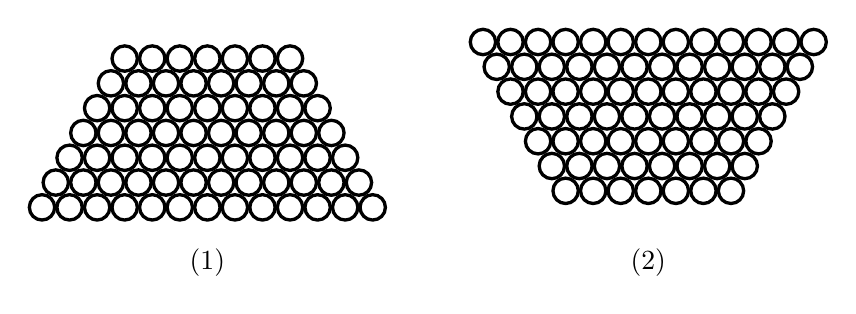
\begin{tikzpicture}[scale=.7]
\begin{scope}
 \foreach \x in {1,2,3,...,13}
{
    \draw[very thick](\x/2,0)circle(.23);
}  
\foreach \x in {1,2,3,...,12}
{
    \draw[very thick](\x/2+.25,.45)circle(.23);
}  
\foreach \x in {1,2,3,...,11}
{
    \draw[very thick](\x/2+.5,.9)circle(.23);
}  
\foreach \x in {1,2,3,...,10}
{
    \draw[very thick](\x/2+.75,.45*3)circle(.23);
}  
\foreach \x in {1,2,3,...,9}
{
    \draw[very thick](\x/2+1,.9*2)circle(.23);
}  
\foreach \x in {1,2,3,...,8}
{
    \draw[very thick](\x/2+1.25,.45*5)circle(.23);
}  
\foreach \x in {1,2,3,...,7}
{
    \draw[very thick](\x/2+1.5,.9*3)circle(.23);
}  
\node at (3.5,-1){(1)};
\end{scope}

\begin{scope}[xshift=8cm]    
\node at (3.5,-1){(2)};

 \foreach \x in {1,2,3,...,13}
{
    \draw[very thick](\x/2,-0+3)circle(.23);
}  
\foreach \x in {1,2,3,...,12}
{
    \draw[very thick](\x/2+.25,-.45+3)circle(.23);
}  
\foreach \x in {1,2,3,...,11}
{
    \draw[very thick](\x/2+.5,3-.9)circle(.23);
}  
\foreach \x in {1,2,3,...,10}
{
    \draw[very thick](\x/2+.75,3-.45*3)circle(.23);
}  
\foreach \x in {1,2,3,...,9}
{
    \draw[very thick](\x/2+1,3-.9*2)circle(.23);
}  
\foreach \x in {1,2,3,...,8}
{
    \draw[very thick](\x/2+1.25,3-.45*5)circle(.23);
}  
\foreach \x in {1,2,3,...,7}
{
    \draw[very thick](\x/2+1.5,3-.9*3)circle(.23);
}  

\end{scope}
\end{tikzpicture}
    \caption{}
\end{figure}


显然,自上而下各层的钢管数排成一个等差数列:7,8、
9、10、11、12、13.

为了求出钢管的总数,我们可以设想如图5.5(2)那样,
在这堆钢管旁边倒放着同样的一堆钢管,把两堆合起来,每
层钢管数都相等,即
\[7+13=8+12=\cdots=13+7\]

由于共有七层,因此两堆钢管总数就是:$(7+13)\x7$,
那么,所求钢管总数是
$$\frac{7+13}{2}\x7=70$$
    
一般地,设有等差数列$a_1,a_2,a_3,\ldots,a_n,\ldots$,
它的前$n$项的和记作$S_n$, 即
\[S_n=a_1+a_2+\cdots+a_n\]
根据等差数列的通项公式,上式可以写成
\[S_n=a_1+(a_1+d)+(a_1+2d)+\cdots+[a_n+(n-1)d]\]

再把项的次序反过来,$S_n$又可以写成
\[S_n=a_n+(a_n-d)+(a_n-2d)+\cdots+[a_n-(n-1)d]\]

将这两个式子相加,得
\[\begin{split}
    2S_n&=\overbrace{(a_1+a_n)+(a_1+a_n)+\cdots +(a_1+a_n)}^{n\text{个}} \\
    &=n(a_1+a_n)
\end{split}\]
由此得到等差数列$\{a_n\}$的\textbf{前$n$项的和的公式}
\begin{equation}
    S_n=\frac{n(a_1+a_n)}{2}\tag{1}
\end{equation}

若将$a_n=a_1+(n-1)d$
代入(1)式,又可得出
\begin{equation}
    S_n=na_1+\frac{n(n-1)}{2}d \tag{2}
\end{equation}

从上述求$S_n$的分析过程可见,在一个等差数列的前$n$项
中,与两端(即$a_1$和$a_n$)“等距离”的两项之和都等于首末两
项之和$a_1+a_n$。这是等差数列所具有的一个重要性质。

公式(1)和公式(2)中,分别含有四个量:$a_1,\; a_n,\;  n,\; S_n$和$a_n,\; d,\; S_n,\; n$。如果已知其中三个量,那么每个公式都可看作以其第四个量为未知数的方程,从而第四个量都可
以求出。

如果再加上前一节学的等差数列的通项公 式$a_n=a_1+$ $(n-1)d$,那么在等差数列中,常涉及到以下五个量:$a_1,\; d,\; n,\; a_n$和$S_n$, 并且它们由一组公式:通项公式 和 前$n$项和公式联系着,因此若已知其中的任何三个量,即可得到以其余两个量为未知数的方程组,从而可以求出其余的两个量。


\begin{example}
    求自然数集合中,前100个自然数的和。
\end{example}

\begin{solution}
前100个自然数,组成首项是1,公差是 1 的等差数
列,共有100项,且第100项是100,所以
$$S_{100}=\frac{1+100}2\times100=5050$$

(这正是著名的德国数学家高斯(1777—1855)在他10
岁时,很快地算出$1+2+\cdots+100$的结果时所用的解法)。 
\end{solution}

\noindent
\begin{minipage}{.55\textwidth}
    \CTEXindent
    \begin{example}
图5.6表示一个堆放
铅笔的V形架,它的最下面一
层放一支铅笔,在上每一层都
比它下面一层多放一支,最上
面一层放120支,问这个V形架
上共放着多少支铅笔?

答案是7260支铅笔,请读者完成计算过程。
\end{example}
\end{minipage}\hfill
\begin{minipage}{.4\textwidth}
\centering
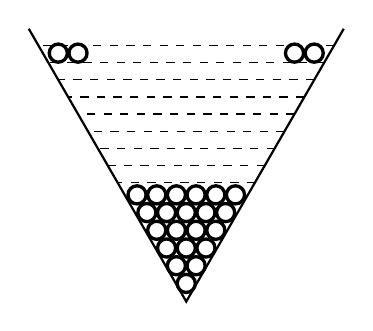
\begin{tikzpicture}[scale=.5]
 \foreach \x in {1,2,3,...,6}
{
    \draw[very thick](\x/2-.5-.25*5,.46+.45*5)circle(.23);
}  
\foreach \x in {1,2,3,...,5}
{
    \draw[very thick](\x/2-.5-.25*4,.46+.45*4)circle(.23);
}  
\foreach \x in {1,2,3,4}
{
    \draw[very thick](\x/2-.5-.25*3,.46+.45*3)circle(.23);
}  
\foreach \x in {1,2,3}
{
    \draw[very thick](\x/2-.5-.25*2,.46+.45*2)circle(.23);
}  
\foreach \x in {1,2}
{
    \draw[very thick](\x/2-.5-.25,.46+.45)circle(.23);
}  
\foreach \x in {1}
{
    \draw[very thick](\x/2-.5,.46)circle(.23);
}  
\draw[thick](120:8)--(0,0)--(60:8);

\foreach \x in {7,8,...,14,15}
{
    \draw[dashed](60:\x/2)--(120:\x/2);
}
\foreach \x in {1,2}
{
    \draw[very thick](\x/2-.5-.25*13,.46+.45*13)circle(.23);
    \draw[very thick](-\x/2+.5+.25*13,.46+.45*13)circle(.23);
}  



\end{tikzpicture}
\captionof{figure}{}
\end{minipage}

\begin{example}
    正偶数组成的数列$2,4,6,\ldots$的前多少项的和等于9900?
\end{example}

\begin{analyze}
    已知:$a_1=2$,公差$d=2$, $S_n=9900$,求$n$。因此,我们利用公式$S_n=n\cdot a_1+\frac{n(n-1)}{2}d$求解。
\end{analyze}

\begin{solution}
    由已知,得
\[n\cdot 2+\frac{n(n-1)}{2}=9900\]
    化简得
\[    n^2+n-9900=0\]
    解得$n=99$或$n=-100$(后者不合题意,舍去)。

    答:数列的前99项之和为9900。
\end{solution}



\begin{example}
求集合$M=\{m\mid m=7n,\; n\in\N,\;  \text{且}m<100\}$中元素的个数,并求这些元素之和。
\end{example}

\begin{solution}
$\because\quad     7n<100$
\qquad\qquad
$\therefore\quad n<\frac{100}{7}=14\frac{2}{7}$

由于满足上面不等式的自然数$n$共有14个,故集合$M$里的元素共14个,将它们从小到大列出,就是
\[7,\quad 7\x2,\quad 7\x3,\; \ldots,\; 7\x14\]
即$7,\;14,\;21,\ldots,98$

这个数列是以首项为7,第14项为$a_{14}=98$的等差数列,因此它们的和为
\[S_{14}=\frac{14(7+98)}{2}=735\]

答:集合$M$里共有14个元素,它们的和为735。
\end{solution}

这个例说明:在100以内的自然数中,共有14个数能被4
7整除,且它们的和为735。


\begin{example}
    有一个凸多边形,它的各内角的度数成等差数列,其最小角为$60^{\circ}$,公差为$20^{\circ}$,求它的边数。
\end{example}

\begin{solution}
    设此多边形的边数为$n$,因为它的内角度数成等差数列,且公差是$20^{\circ}$,第一个角是$60^{\circ}$,所以
\[S_n=n\cdot 60+\frac{n(n-1)}{2}\cdot 20\]

另一方面,凸多边形内角和为$(n-2)\cdot 180^{\circ}$,所以
\[n\cdot 60+n(x-1)\cdot 20=(m-2)\cdot 180\]
化简整理,得
\[n^2-13n+36=0\]
解之,得
$n=4$,或$n=9$.

若$n=9$,则$a_9=a_1+(9-1)\cdot d=60+8\x20>180$, 
所以$n=9$不合题意,应舍去。

答:这个多边形的边数是4。
\end{solution}

观察公式,
$S_n=na_1+\frac{n(n-1)}{2}d$是项数$n$的二次型
代数式,我们有下面的定理

\begin{thm}
    {定理2} 设数列$\{a_n\}$的前$n$项和为$S_n$,求证数列$\{a_n\}$是等差数列的充要条件是$S_n=an^2+bn$(其中$a$,$b$为已知常数)。
\end{thm}

\begin{proof}
    先证“必要性”,即证“若$\{a_n\}$是等差数列,则$S_n=a\cdot n^2+bn$.”证明如下:

$\because\quad \{a_n\}$ 是等差数列,

$\therefore\quad S_n=na_1+\frac{n(n-1)}{2}d=\frac{d}{2}n^2+\left(a_1-\frac{d}{2}\right)n$

只需令$\frac{d}{2}=a,\quad a_1-\frac{d}{2}=b$,则有$S_n=an^2+bn$.

再证“充分性”,即证“若数列的前$n$项和$S_n=an^2+bn$,则$\{a_n\}$是等差数列”,证明如下:
$\because\quad S_n=an^2+bn$

$\therefore\quad a_n=\begin{cases}
    S_n-S_{n-1}=2an-a+b, & n\ge 2\\
    S_1=a+b, & n=1
\end{cases}$

$\because\quad n=1$时,$2an-a+b=a+b=S_1$

$\therefore\quad $数列$\{a_n\}$的通项公式为$a_n=2an-a+b\; (n\ge 1)$,由定理1,$\{a_n\}$是等差数列。
\end{proof}


\begin{example}
    设$\{a_n\}$为等差数列,且$S_{10}=100$, $S_{100}=10$,试求前110项之和$S_{110}$.
\end{example}

\begin{analyze}
解法之一是,利用等差数列的求和公式$S_n=a_n+\frac{n(n-1)}{2}d$
,及条件$S_{10}=100$, $S_{100}=10$,列出关于$a_1$与$d$的二元方程组,解出$a_1$与$d$来,然后再求$S_{110}$(请读者自己来完成).

解法之二是,利用定理2,可设$S_n=an^2+bn$,依据条件用待定系数法求出$a$与$b$来,再求$S_{110}$。
\end{analyze}

\begin{solution}
因为$\{a_n\}$为等差数列,由定理2可设$S_n=an^2+bn$,由已知,有
\[\begin{cases}
    a\cdot 10^2+b\cdot 10=100\\
    a\cdot 100^2+b\cdot 100=10
\end{cases}\]
解之,得
$\begin{cases}
    a=-\frac{11}{100}\\[1.5ex]
    b=\frac{111}{10}
\end{cases}$

$\therefore\quad S_{110}=-\frac{11}{100}\x 110^2+\frac{111}{10}\x 110=-110$
\end{solution}



\begin{example}
    已知等差数列中,$a_3+a_{18}=100$,求$S_{20}$.
\end{example}

\begin{solution}
$\because\quad a_3+a_{18}=a_1+a_{20}=100$

$\therefore\quad S_{20}=\frac{a_1+a_{20}}{2}\x20=\frac{100}{2}\x 20=1000$.
\end{solution}


\begin{example}
    已知等差数列$\{a_n\}$的通项公式为$a_n=3n-26$,求其前$n$项和$S_n$的最大值或最小值。
\end{example}

\begin{solution}
 $\because\quad    a_1=3\x 1-26=-23<0,\quad d=3>0$

 $\therefore\quad S_n$有最小值,无最大值。

 设$a_n=3n-26\le 0$,得
\[n\le \frac{26}{3}=8\frac{2}{3}\]
即数列的前8项均为负数,而第9项$a_9=3\x9-26=1>0$,故前8项之和$S_8$是$S_n$的最小值。其最小值为
\[S_8=8\x(-23)+\frac{8\x7}{2}\x3=-100\]
\end{solution}

\begin{example}
    已知等差数列$\{a_n\}$中,$a_n=32$,公差为$-4$,求它的前$n$项和$S_n$的最大值或最小值。
\end{example}

\begin{solution}
    因为$a_1=32$, $d=-4<0$,所以数列的前$n$项和$S_n$有最大值,无最小值。

    设$a_n=32+(n-1)\x(-4)\ge 0$, 求得$n\le 9$, 
即数列的前9项为非负数,而第10项开始为负数,又$a_0=0$, 所以前8项的和与前9项的和相等,即$S_8=S_9$,且它们是$S_n$的最大值,最大值是:
\[S_8=32\x8+\frac{8\x7}{2}\x(-4)=144\]
或
\[S_9=32\x9+\frac{9\x8}{2}\x(-4)=144\]

\textbf{另解:}因为等差数列前$n$项和$S_n$当$d\ne 0$时是$n$的二次式,所以也可以借助于求二次函数的极值的方法,来求$S_n$的最大值或最小值。

如例5.16中,$a_n=3n-26$,所以$a_1=-23$,于是
\[\begin{split}
    S_n=\frac{n(-23+3n-26)}{2}&=\frac{3}{2}n^2-\frac{49}{2}n\\
    &=\frac{3}{2}\left(n-\frac{49}{6}\right)^2-\frac{3}{2}\x \left(\frac{49}{6}\right)^2
\end{split}\]
然而,这里$n\in\N$,所以$n-\frac{49}{6}\ne 0$,只有当$\left|n-\frac{49}{6}\right|$最小时,即$n=8$时,$S_n$取得最小值,此时,$(S_n)_{\min}=\frac{3}{2}\x 8^2-\frac{49}{2}\x 8=-100$

又如例5.17中,有
\[\begin{split}
    S_n=\frac{n(32+32-4n-4)}{2}&=-2n^2+34n\\
    &=-2\left(n-\frac{17}{2}\right)^2+2\x \left(\frac{17}{2}\right)^2
\end{split}\]
当$\left|n-\frac{49}{6}\right|$最小,即$n=8$或$n=9$时,$S_n$取得最大值144.
\end{solution}

\begin{example}
    求数列$\left\{\lg\left(1000\sin^n\frac{\pi}{4}\right)\right\}$的前$n$项之和$S_n$的最大值.
\end{example}

\begin{solution}
\[\begin{split}
\because\quad a_n-a_{n-1}=\lg1000\sin^n\frac{\pi}{4}-\lg1000\sin^{n-1}\frac{\pi}{4}   
&=\lg\frac{1000\sin^n\frac{\pi}{4}}{1000\sin^{n-1}\frac{\pi}{4}}\\
&=\lg\sin\frac{\pi}{4}=-\frac{1}{2}\lg 2
\end{split}\]

$\therefore\quad $该数列是等差数列,其公差为$-\frac{1}{2}\lg 2$,首项$a_1=\lg1000 \sin\frac{\pi}{4}=3-\frac{1}{2}\lg2$. 因为$a_i>0$, $d<0$,故$S_n$有最大值。

设$a_n=\lg 1000\sin^n\frac{\pi}{4}\ge 0$, 得
\[3-\frac{n}{2}\lg2\ge 0\quad \Rightarrow\quad n\le \frac{6}{\lg 2}\approx 19.9\]

答:$S_{19}$是$S_n$的最大值,其值$S_{19}\approx 28.40$.

(读者可利用另一种方法求其最大值)
\end{solution}

\begin{ex}
\begin{enumerate}
    \item 根据下列各题的条件,求相应的等差数列{am}的前n项和"S
\begin{enumerate}[(1)]
 \item $a_1=5,\quad a_n=65,\quad n=10$;
\item $a_1=100,\quad d=-2,\quad n=50$;
\item $a_1=\frac{2}{3},\quad a_n=-\frac{3}{2},\quad n=14$;
\item $a_1=14.5,\quad d=0.7,\quad a_n=32$.   
\end{enumerate}

    \item \begin{enumerate}[(1)]
        \item 求自然数列中前100个奇数的和;
        \item 求前100个自然数中,所有被3除余2的自然数的个数,以及它们的和;
        \item 两位自然数中被7除余1的各数之和。
    \end{enumerate} 

    \item 根据下列各题中的条件,求相应的等差数列$\{a_n\}$中的有关未知数:
\begin{enumerate}[(1)]
    \item $a_1=20,\quad a_n=54,\quad S_n=999$,求$d$和$n$;
\item $d=\frac{1}{3},\quad n=37,\quad S_n=629$,求$a_1$和$a_n$;
\item $a_1=\frac{5}{6},\quad d=-\frac{1}{6},\quad S_n=-5$,求$n$和$a_n$;
\item $d=2,\quad n=15,\quad a_n=-10$,求$a_1$和$S_n$.
\end{enumerate}
\item \begin{enumerate}[(1)]
\item 在正整数集合里,有多少个三位数,并求出它们的和;
\item 在三位正整数的集合中有多少个数是7的整数倍?并求它们的和,
\item 求等差数列$13,15,17,\ldots,81$的各项之和;
\item 求等差数列$10,7,4,\ldots,-47$的各项之和。
\end{enumerate}
\item 根据下列条件,求数列前多少项的和最大(或最小),并求出其最大值或最小值.
\begin{enumerate}[(1)]
    \item $\{a_n\}$是等差数列,且
\begin{multicols}{2}
\begin{enumerate}[(a)]
    \item $a_2=7,\quad a_6=23$;
    \item $a_{20}=-1,\quad d=-\frac{1}{2}$.
\end{enumerate}
\end{multicols}

\item 数列$\{a_n\}$的通项公式是
\begin{multicols}{2}
    \begin{enumerate}[(a)]
        \item $a_n=-5n+2$;
        \item $a_n=33-3n$.
    \end{enumerate}
    \end{multicols}

\item 数列$\{a_n\}$的前$n$项和为 $S_n=2n^2-23n+\frac{123}{2}$
\end{enumerate}
\end{enumerate}
\end{ex}

\section*{习题二}
\begin{center}
    \bfseries A
\end{center}

\begin{enumerate}
    \item 已知数列$\{a_n\}$是等差数列。
\begin{enumerate}[(1)]
\item 若$a_2+a_9+a_{12}+a_{19}=100$,求$S_{20}$;
\item 若$a_{10}=20$,求$S_{19}$;
\item 若$a_4=7$, $a_9=5$,求$a_{19}$和$a_{20}$.
\end{enumerate}

    \item 三个数成等差数列,它们的和等于18,它们的平方和等于116,求这三个数。
    \item  \begin{enumerate}[(1)]
        \item 某等差数列$\{a_n\}$的通项公式是$a_n=3n-2$,求它的前$n$项和;
    \item 某等差数列$\{a_n\}$的前$n$项和公式是$S_n=5n^2+3n$,求它的前3项及通项公式。
    \end{enumerate}   
    \item     一个等差数列的第6项是5,第3项与第8项之和也是5,求该数列的前9项之和。
    \item     一个屋顶的某一斜面成等腰梯形,最上面一层铺了瓦片21块,往下每一层多铺一块,斜面上共铺了瓦片19层,共铺了多少块瓦?
    \item     一个剧场设置了20排座位,第一排38个座位,往后每一排比前一排多2个座位。这个剧场一共设置了多少个座位?
\item \begin{enumerate}[(1)]
    \item 一个等差数列的第1项是5.6,第6项是20.6,求它的第四项。
    \item  一个等差数列第3项是9,第9项是3,求它的第2项。
    \item 一个等差数列第5项是$5a-b$,第2项是$2a+2b$,求第3项和第6项。
    \end{enumerate}
\item \begin{enumerate}[(1)]
\item 在12和60之间,插入3个数,使这5个数构成等差数列,求这三个数。
\item 在8和36之间插入6个数,使这8个数构成等差数列,求这六个数。
\item 在$a$和$b$之间插入10个数,使这12个数构成等差数列,求这个数列的第六项。
\end{enumerate}
\item 在通常情况下,从地面到1万米高空,高度每增加1千米,气温就下降某一固定数值。如果1千米高度的气温是$8.5^{\circ}{\rm C}$,5千米高度的气温是$-17.5^{\circ}{\rm C}$。求2千米、4千米及8千米高度的气温。
\item 安装在一个公共轴上的5个皮带轮的直径成等差数列,其中最大的与最小的皮带轮直径分别是216毫米与120毫米,求中间三个皮带轮的直径。

\end{enumerate}





\begin{center}
    \bfseries B
\end{center}

\begin{enumerate}\setcounter{enumi}{10}
    \item  某多边形的周长等于195cm,所有各边的长成等差数列,最大的边长等于40cm,公差是3cm,求多边形的边数。
    \item  一个梯形两条底边的长分别是12cm和22cm,将梯形的一条腰10等分,过每个分点画平行于梯形底边的直线,求这些直线夹在梯形两腰间的线段的长度之和。
    \item  长方体的三条棱的长成等差数列,它的对角线的长是$5\sqrt{2}$cm,全面积是$94{\rm cm^2}$,求它的体积。
    \item  一个凸多边形的各内角的度数成等差数列,其公差为$5^{\circ}$,又最小内角是$120^{\circ}$,求这个多边形的边数。
    \item 已知数$\lg1000,\; \lg1000\cos\frac{\pi}{3},\; \lg1000\cos^2 \frac{\pi}{3},\ldots, 
    \lg1000\cos^{n-1}\frac{\pi}{3},\ldots$的前多少项的和最大,并求出其
    最大值。
\end{enumerate}

\section*{三、等比数列}
\section{等比数列的有关概念}
观察下面的数列:
\begin{align}
 &1,\; 2,\; 4,\; 8,\; 16,\ldots  \tag{1}\\
&5,\; 5,\; 5,\; 5,\ldots\tag{2}\\
&1,\; -\frac{1}{2},\; \frac{1}{4},\; -\frac{1}{8},\; \frac{1}{16},\;\ldots \tag{3}   
\end{align}

\begin{itemize}
\item 数列(1)中,从第2项起每一项与前一项的比都等于2;
\item 数列(2)中,从第2项起每一项与前一项的比都等于1;
\item 数列(3)中,以第2项起每一项与前一项的比都等于$-\frac{1}{2}$.
\end{itemize}

它们的共同特点是:以第2项起,每一项与它的前一项之比都等于同一个非零常数,通常把这个常数记作$q$,即
\[\frac{a_n}{a_{n-1}}=q\quad (n\ge 2,\; n\in\N,\; q\text{为常数},\; q\ne 0)\]
这类数列叫做\textbf{等比数例},常数$q$叫做等比数列的\textbf{公比}。上述三个等比数列的公比分别是2, 1和$-\frac{1}{2}$.数列(2)说明一个非零常数列一定是等比数列,且它的公比为1。

由等比数列的定义可知,一个等比数列中的任何一项都不能是零。

如果有三个数$x$、$G$、$y$组成等比数列,那么$G$叫做$x$和$y$的\textbf{等比中项}。

根据等比数列的定义可知$\frac{G}{x}=\frac{y}{G}$,所以$G^2=xy$,
因此$G=\pm\sqrt{xy}$.

由此可知,在实数集合内,只有当$x$与$y$是同号的两个数时,它们才有等比中项,当两个数有等比中项时,必有两个等比中项,且它们互为相反数。

容易看出,在一个无穷的等比数列中,从第2项起,每一项都是它的前一项与后一项的等比中项。


\begin{example}
已知数列的通项公式为$a_n=\frac{1}{3}\x 2^n$,求证:
\begin{enumerate}[(1)]
\item 数列$\{a_n\}$是等比数列,并求其公比;
\item 求出数列的首项及第10项;
\item 判断256和$170\frac{2}{3}$是不是该数列中的项。如果是,是第几项?
\end{enumerate}
\end{example}

\begin{solution}
\begin{enumerate}[(1)]
    \item $\because\quad \frac{a_n}{a_{n-1}}=\frac{\frac{1}{3}\x 2^n}{\frac{1}{3}\x 2^{n-1}}=2$(常数)
    
$\therefore\quad $数列是等比数列,且公比是2。
\item 首项$a_1=\frac{1}{3}\x2=\frac{2}{3}$, $a_{10}=\frac{1}{3}\x2^{10}=\frac{1024}{3}$.
\item 设$a_n=\frac{1}{3}\x2^n=259$,则$n=8+\log_2 3$不是整数,所以256不是数列中的项。

设$a_n=\frac{1}{3}\x2^n=170\frac{2}{3}=\frac{512}{3}$则$n=9$,所以$170\frac{2}{3}$是
该数列的第9项。
\end{enumerate}
\end{solution}


\section{等比数列的通项公式}
如果等比数列$\{a_n\}$的第一项为$a_1$,公比为$q$,那么根据等比数列的定义得
\[\begin{split}
  a_2&=a_1q,\\
a_3&=a_2q=(a_1q)q=a_1q^2,\\
a_4&=a_3q=(a_1q^2)q=a_1q^3.\\  
\cdots &\cdots \cdots \cdots \cdots \cdots 
\end{split}\]

由此我们可以归纳出,数列的通项公式是
\[a_n=a_1q^{n-1}\quad (a_1\ne 0,\; q\ne 0)\]
其正确性,可用数学归纳法给予证明。

上面的公式还可用下面的方法得到:
\[\begin{split}
    a_1&=a_1\\
    \frac{a_2}{a_1}&=q\\
    \frac{a_3}{a_2}&=q\\
    \cdots&\cdots\cdots\\
    \frac{a_{n-1}}{a_{n-2}}&=q\\
    \frac{a_n}{a_{n-1}}&=q
\end{split}\]
将这$n$个等式的等号两边分别相乘,即可得出
\[a_n=a_1q^{n-1}\]
上面这个方法,称之为\textbf{迭乘法}。

等比数列通项公式还可以改写成
\[a_n=\frac{a_1}{q}\cdot q^n=cq^n\]
其中$c=\frac{a_1}{q}$,是一个不为零的常数。

要确定函数$y=c\cdot q^x$需要两个独立条件,因此要确定等比数列的通项公式,也需要两个独立条件。

\begin{example}
    求等比数列$\frac{\sqrt{2}}{2},\; -1,\; \sqrt{2},\; -2,\ldots$的第100项。
\end{example}

\begin{solution}
$\because\quad a_1=\frac{\sqrt{2}}{2},\quad q=-\sqrt{2}$

$\therefore\quad a_{100}=\frac{\sqrt{2}}{2}\cdot \left(-\sqrt{2}\right)^{100-1}=-\frac{\sqrt{2}}{2}\cdot \left(\sqrt{2}\right)^{99}=-2^{49}$
\end{solution}

\begin{example}
    一个等比数列的第3项与第4项分别是12与18,求它的第1项,第2项,和它的通项公式。
\end{example}

\begin{solution}
设这个数列为$\{a_n\}$,则它的公比
\[q=\frac{a_4}{a_3}=\frac{18}{12}=\frac{3}{2}\]

$\because\quad a_3=a_2\cdot q=a_2\cdot \frac{3}{2}=12$

$\therefore\quad a_2=8$

$\because\quad a_2=a_1q=a_1\cdot \frac{3}{2}=8$

$\therefore\quad a_1=\frac{16}{3},\quad a_n=a_1\cdot q^{n-1}=\frac{16}{3}\cdot \left(\frac{3}{2}\right)^{n-1}=2^{5-n}\cdot 3^{n-2}$
\end{solution}



\begin{example}
    培育水稻新品种,如果得到第一代120粒种子,并且从第一代起,以后各代的每一粒种子都可以得到下一代的120粒种子,到第五代大约可以得到这种新品种的种子多少粒(保留两位有效数字)?
\end{example}

\begin{solution}
由于每代的种子数是它的前一代种子数的120倍,逐代的种子数组成等比数列,记作$\{a_n\}$,其中$a_1=120$, $q=120$, 因此
\[a_5=120\x120^{5-1}\approx 2.5\x10^{10}\]
答:到第五代大约可以得到种子$2.5\x10^{10}$粒。
\end{solution}

    
\begin{example}
    求证数列$\{a_n\}$(其中$a_k\ne 0,\; k=1,2,\ldots$)是等比
数列的充要条件是其通项公式为$a_n=c\cdot q^n$(其中$c$、$q$均为非零常数).
\end{example}

\begin{proof}
先证“充分性”,即证“若$a_n=c\cdot q^n$,则$\{a_n\}$成等比数列”,证明如下:

$\because\quad a_n=c\cdot q^n\quad (cq\ne 0)$

$\therefore\quad \frac{a_n}{a_{n-1}}=\frac{c\cdot q^n}{c\cdot q^{n-1}}=q$(非零常数),

$\therefore\quad \{a_n\}$是等比数列。

再证“必要性”,即“若$\{a_n\}$成等比数列,则$a_n=cq^n$”.

$\because\quad\{a_n\}$成等比数列,

$\therefore\quad a_n=a_1\cdot q^{n-1}=\frac{a_1}{q}\cdot q^n$

令$c=\frac{a_1}{q}$,即得到$a_n=c\cdot q^n$·

综上可知,$\{a_n\}$成等比数列的充要条件$a_n=c\cdot q^n\quad (cq\ne 0)$
\end{proof}

\begin{example}
    在1和8之间插入5个数,使得这7个数组成等比数列,试求插入的5个数。
\end{example}

\begin{solution}
    设数列的公比为$q$. 由$a_1=1$得
\[a_7=8=a_1 q^6=q^5\]
$\therefore\quad q=\pm\sqrt{2}$

答:插入的5个数是$\sqrt{2},\; 2,\; 2\sqrt{2},\; 4,\; 4\sqrt{2}$或$-\sqrt{2},\; 2,\; -2\sqrt{2},\; 4,\; -4\sqrt{2}$.
\end{solution}

\begin{example}
    已知$\{a_n\}$为等比数列,公比为$q$,求证
$a_n=a_mq^{n-m}$.
\end{example}

\begin{proof}
    由等比数列通项公式,得
\[a_n=a_1q^{n-1},\qquad a_m=a_1q^{m-1}\]

$\therefore\quad a_n=a_1q^{m-1}\cdot q^{n-m}=a_m q^{n-m}$
\end{proof}


\begin{example}
    已知$\{a_n\}$为等比数列且$a_m=16$, $a_{m+4}=9$,求数列的通项公式。
\end{example}

\begin{solution}
设数列的公比为$q$,则$a_{m+4}=a_m q^4$,即
\[q^4=\frac{9}{16}\quad \Rightarrow\quad q=\pm\frac{\sqrt{3}}{2}\]

$\therefore\quad a_n=a_m\cdot q^{n-m}=16\x \left(\pm\frac{\sqrt{3}}{2}\right)^{n-m}$
\end{solution}


\begin{example}
    设$\{a_n\}$为等比数列。$k,\ell,m,n\in\N$,若$k+\ell=m+n$,则$a_k\cdot a_{\ell}=a_m\cdot a_n$
\end{example}

\begin{proof}
    设公比为$q$,则
\[\begin{split}
    a_{k}\cdot a_{\ell}&=a_1q^{k-1}\cdot a_1q^{\ell-1}=a^2_1\cdot q^{k+\ell-2}\\
    a_{m}\cdot a_{n}&=a_1q^{m-1}\cdot a_1q^{n-1}=a^2_1\cdot q^{m+n-2}\\
\end{split}\]

$\because\quad k+\ell=m+n$

$\therefore\quad a_k\cdot a_{\ell}=a_m\cdot a_n$
\end{proof}

\begin{rmk}
    此例说明,在等比数列中,当两项的项数和与另两项项数和相等时,对应的两项之积也相等。这是等比数列的重要性质之一。

特别地,$a_1\cdot a_n=a_2\cdot a_{n-1}=a_3\cdot a_{n-2}=\cdots$.
\end{rmk}

\begin{ex}
\begin{enumerate}
    \item 解下列各题:
\begin{enumerate}[(1)]
\item 求等比数列$5,\; -15,\; 45,\;\ldots$的第4项,第5项;
\item 求等比数列$\frac{2}{3},\; \frac{1}{2},\; \frac{3}{8},\;\ldots$的第6项;
\item 求等比数列$\sqrt{2},\; 1,\; \frac{\sqrt{2}}{2},\; \ldots$的第$n$项;
\item 求等比数列$1,\; -\frac{1}{2},\; \frac{1}{4},\; \ldots$的第$n+1$项。
\end{enumerate}

\item 在等比数列$\{a_n\}$中,设公比为$q$.
\begin{enumerate}[(1)]
\item 已知$a_9=\frac{4}{9},\quad q=-\frac{1}{3}$, 求$a_1$;
\item 已知$a_2=10,\quad a_3=20$,求$a_n$;
\item 已知$a_2=2,\quad a_5=54$,求$q$;
\item 已知$a_1=1,\quad a_n=256,\quad q=2$,求$n$;
\item 已知$a_4=27,\quad q=-3$,求$a_7$;
\item 已知$a_5-a_1=15,\quad a_4-a_2=6$,求$a_n$.
\end{enumerate}

\item 求下列各组数的等比中项。
\begin{enumerate}[(1)]
\item 45与80
\item $9\frac{3}{8}$与$1\frac{1}{2}$
\item $7+3\sqrt{5}$与$7-3\sqrt{5}$
\item $a^4+a^2b^2$与$b^4+a^2b^2\quad (2b\ne 0)$
\end{enumerate}

\item \begin{enumerate}[(1)]
\item 在9和243之间插入两个数,使它们同这两个数成等比数列;
\item 在160和5之间插入4个数,使它们同这两个数成等比数列。  
\end{enumerate}

\item 某林场计划第一年造林80亩,以后每一年比前一年多造林20\%,第五年造林多少亩(保留到个位)?
\end{enumerate}
\end{ex}

\section{等比数列前$n$项的和}
设等比数列$\{a_n\}$的公比为$q$,首项为$a_1$,由等比数列的定
义,有
\[\begin{split}
    a_2&=a_1q\\
    a_3&=a_2q\\
    a_4&=a_3q\\
    \cdots&\cdots\cdots\\
    a_{n-1}&=a_{n-2}q\\
    a_n &=a_{n-1}q
\end{split}\]
将上述$n-1\; (n\ge 2)$个等式的等号两边分别相加,得
\[a_2+a_3+\cdots +a_n=q(a_1+a_2+\cdots +a_{n-1})\]
即
\[\begin{split}
S_n-a_1&=q(S_n-a_n)\\
(1-q)S&=a_1-a_nq     
\end{split}\]
当$q\ne 1$时,$$S_n=\frac{a_1-a_n q}{1-q}$$
上式对$n=1$显然成立。

当$q=1$时,$S_n=a_1+a_2+\cdots +a_n=na_1$,这样就得出等比数列前$n$项和公式
\begin{equation}
    S_n=\begin{cases}
        na_1,  & q=1\\[1.5ex]
        \frac{a_1-a_nq}{1-q},& q\ne 1
    \end{cases}\tag{1}
\end{equation}

将等比数列的通项公式$a_n=a_1q^{n-1}$代入,可得
\begin{equation}
    S_n=\begin{cases}
        na_1,  & q=1\\[1.5ex]
        \frac{a_1(1-q^n)}{1-q},& q\ne 1
    \end{cases}\tag{2}
\end{equation}
公式(2)中$q\ne 1$时的结论还可以用下面的方法得到,设
\begin{equation}
    S_n=a_1+a_2q+a_3q^2+\cdots+a_1q^{n-2}+a_1q^{n-1} \tag{*}
\end{equation}
将上式中各项都乘以$q$,便得到
\begin{equation}
  qS_n=a_1q+a_1q^2+\cdots+a_1q^{n-1}+a_1q^n \tag{**}  
\end{equation}

比较上述两式的右端,可见,(*)的右式中,从第2项至第$n$项与(**)式右端的第1项至第$n-1$项完全相同,因此,以(*)式两边分别减去(**)式两边,便可得到
\[(1-q)S_n=a_1-a_1q^n\]
从而得出
\[S_n=\frac{a_1(1-q^n)}{1-q}\quad (q\ne 1)\]

等比数列的前$n$项和公式(1)和(2),及等比数列的通项公式$a_n=a_1q^{n-1}$其中涉及$a_1, q, n, a_n$和$S_n$这5个量。而它们又通过通项公式及前$n$项和公式联系着,因此只要已知其中的任何三个量,即可得到以其余两个量为未知数的方程组,从而可以求出其余两个量。

\begin{example}
    求等比数列$\frac{1}{2},\; \frac{1}{4},\; \frac{1}{8},\; \ldots$的第10项及前10项之和。
\end{example}

\begin{solution}
已知$a_1=\frac{1}{2},\quad q=\frac{1}{2},\quad n=10$
\[\therefore\quad a_{10}=a_1q^{10-1}=\frac{1}{2}\cdot \left(\frac{1}{2}\right)^9=\frac{1}{1024},\qquad 
S_{10}=\frac{\frac{1}{2}\left(1-\frac{1}{2^{10}}\right)}{1-\frac{1}{2}}=\frac{1023}{1024}\]
\end{solution}

\begin{example}
     某制糖厂今年制糖5万吨,如果平均每年的产量比上一年增加10%,那么从今年起,几年内可以使总产量达到30万吨(保留到个位)?
\end{example}

\begin{solution}
由题意可知,这个糖厂从今年起,平均每年的产量(万吨)组成一个等比数列,记为$\{a_n\}$,其中
\[a_1=5,\quad q=1+10\%=1.1,\quad S_n=30\]
于是得到
\[\frac{5(1-1.1^n)}{1-1.1}=30\]

整理后,得
\[1.1^n=1.6\]
两边取对数,得
\[n\lg 1.1=\lg 1.6\]

$\therefore\quad n=\frac{\lg 1.6}{\lg 1.1}=\frac{0.2041}{0.0414}\approx 5$

答:5年内可以使总产量达到30万吨。
\end{solution}

\begin{example}
    已知无穷数列
$10^{\tfrac{0}{5}},\; 10^{\tfrac{1}{5}},\; 10^{\tfrac{2}{5}},\; \ldots,10^{\tfrac{n-1}{5}},\ldots$
求证:
\begin{enumerate}[(1)]
\item 这个数列是等比数列;
\item 这个数列中任意一项是它后面第5项的$\frac{1}{10}$;
\item 这个数列中任意两项的积仍然在这个数列中;
\item 求该数列的前$n$项之积。
\end{enumerate}
\end{example}

\begin{solution}
\begin{enumerate}[(1)]
    \item 这个数列中的第$n$项与第$n+1$项分别是
$10^{\tfrac{n-1}{5}}$与$10^{\tfrac{n}{5}}\; (n\ge 1)$,于是$n+1$项与第$n$项的比为
\[\frac{a_{n+1}}{a_n}=\frac{10^{\tfrac{n}{5}}}{10^{\tfrac{n-1}{5}}}=10^{\tfrac{n}{5}-\tfrac{n-1}{5}}=10^{\tfrac{1}{5}}\]
即它们的比值是常数$10^{\tfrac{1}{5}}$,因此这个数是以$10^{\tfrac{1}{5}}$为公比的等比数列。

\item 这个数列的第$n$项$a_n=10^{\tfrac{n-1}{5}}$,第$n+5$项$a_{n+5}=10^{\tfrac{n+5-1}{5}}=10^{\tfrac{n+4}{5}}$,于是
\[\frac{a_n}{a_{n+5}}=\frac{10^{\tfrac{n-1}{5}}}{10^{\tfrac{n+4}{5}}}=10^{\tfrac{n-1}{5}-\tfrac{n+4}{5}}=10^{-\tfrac{5}{5}}=10^{-1}=\frac{1}{10}\]

这说明,这个数列中的任意一项,每经过5项后,就变大为原来的10倍,例如$a_8=10\cdot a_3,\; a_{19}=10\cdot a_{14}$等。

\item 从该数列中任取两项,假设它们分别是$a_{n_1}$和$a_{n_2}$,则$a_{n_1}=10^{\tfrac{n_1-1}{5}}$, $a_{n_2}=10^{\tfrac{n_2-1}{5}}$(其中$n_1,n_2\in\N$),那么
\[a_{n_1}\cdot a_{n_2}=10^{\tfrac{n_1-1}{5}}\cdot 10^{\tfrac{n_2-1}{5}}=10^{\tfrac{n_1-1}{5}+\tfrac{n_2-1}{5}}=10^{\tfrac{(n_1+n_2-1)-1}{5}}\]

因为$n_1\ge 1$, $n_2\ge 1$, $n_1\ne n_2$,所以$n_1+n_2>2$,即
\[n_1+n_2-1>1\]
又因为$n_1,n_2\in\N$,所以$n_1+n_2-1\in\N$,这就说明$10^{\tfrac{(n_1+n_2-1)-1}{5}}$是数列的第$n_1+n_2-1$项
\item 
\[\begin{split}
    a_1\cdot a_2\cdots a_n&=10^{\tfrac{0}{5}}\cdot 10^{\tfrac{1}{5}}\cdots 10^{\tfrac{n-1}{5}}\\
    &=10^{\tfrac{0}{5}+\tfrac{1}{5}+\cdots+\tfrac{n-1}{5}}\\&=10^{\tfrac{1}{5}\cdot \tfrac{0+n-1}{2}\cdot n}=10^{\tfrac{n^2-n}{10}}
\end{split}\]
\end{enumerate}
\end{solution}

\begin{ex}
\begin{enumerate}
    \item 根据下列条件,求相应的等比数列$\{a_n\}$的前$n$项和$S_n$:
\begin{enumerate}[(1)]
\item $a_1=3,\; q=2,\; n=6$;
\item $a_1=2.4,\; q=-1.5,\; n=5$;
\item $a_1=8,\; q=\frac{1}{2},\; n=5$;
\item $a_1=-27,\; q=-\frac{1}{3},\; n=6$.
\end{enumerate}

    \item \begin{enumerate}[(1)]
    \item 求等比数列$1,\;2,\;4,\ldots$从第5项到第10项的和;
    \item 求等比数列$\frac{3}{2},\; \frac{3}{4},\; \frac{3}{8},\ldots$从第3项到第7项的和.   
    \end{enumerate}

    \item    在等比数列$\{a_n\}$中
\begin{enumerate}[(1)]
\item 已知$a_1=-1.5$, $a_4=96$,求$q$及$S_4$;
\item 已知$q=\frac{1}{2}$, $S_6=3\frac{7}{8}$, 求$a_1$与$a_5$;
\item 已知$a_1=2$, $S_3=26$,求$q$与$a_3$;
\item 已知$a_3=1\frac{1}{2}$,$S_3=4\frac{1}{2}$,求$a_1$与$q$.   
\end{enumerate}

\end{enumerate}
\end{ex}

\section*{习题三}
\begin{center}
    \bfseries A
\end{center}

\begin{enumerate}
    \item 在等比数列$\{a_n\}$中:
\begin{multicols}{2}
 \begin{enumerate}[(1)]
    \item 已知$n$,$q$,$a_n$,求$a_1$与$S_n$
    \item 已知$q$,$n$,$S_n$,求$a_1$与$a_n$
    \item 已知$a_1$,$q$,$S_n$,求$a_n$
    \item 已知$q$,$a_n$,$S_n$,求$a_1$
\end{enumerate}   
\end{multicols}
\item 某工厂去年的产值是138万元,计划在今后5年内每年比上一年产值增长10\%。从今年起,到第5年这个厂的年产值是多少?这5年的总产值是多少(精确到万元)?
\item 画一个边长为2cm的正方形,再以这个正方形的对角线为边画第二个正方形,以第二个正方形的对角线为边画第3个正方形,这样一共画了10个正方形。求:
\begin{multicols}{2}
\begin{enumerate}[(1)]
\item 第10个正方形的面积;
\item 这10个正方形的面积之和。
\end{enumerate}
\end{multicols}
\item 一个球从100米高处自由落下,每次着地后又跳回到原来高度的一半再落下。当它第10次着地时,共经过了多少米(保留到个位)?
\item 从盛满20升纯酒精的容器里倒出1升,然后用水填满,再倒出1升混合液,用水填满,这样继续进行,一共倒了3次,这时容器里还有多少升纯酒精(保留到个位)?
\item 三个数成等比数列,它们的和等于14,它们的积等于64,求这三个数。
\item 抽气机的活塞每运动一次,从容器里抽出$\frac{1}{8}$的空气,因而使容器里空气的压强降低为原来的$\frac{7}{8}$,已知最初容器里空气的压强是750毫米高水银柱,求活塞运动5次后容器里空气的压强(保留到个位)。
\item 某种细菌在培养过程中,每30分钟分裂一次(一个分裂为两个),经过4小时,这种细菌由1个可繁殖成多少个?电动机轴的直径从小到大共有5种尺寸,它们的数值(单位:mm)组成一个等比数列,其中最小的数值为40,最大的数值为100,求它们的公比(保留到千分位)。
\item 一个工厂今年生产某种机器1080台,计划到后年把产量提高到每年生产机器1920台,如果每一年比上一年增长的百分率相等,求这个百分率(精确到1\%)。
\end{enumerate}

\begin{center}
    \bfseries B
\end{center}

\begin{enumerate}\setcounter{enumi}{10}
    \item 设等比数列$\{a_n\}$的公比是$q$,求证:
    $a_1a_2\cdots a_n=a^n_1q^{\tfrac{n(n-1)}{2}}$
    \item 一个等比数列的各项都是正数,求证这个数列的各项的对数组成等差数列。
    \item 已知$a_1,a_2,a_3,\ldots$是等差数列,$C$是正的常数,求证$C^{a_1},C^{a_2},C^{a_3},\ldots$是等比数列。
    \item 成等差数列的三个正数之和是15,并且将这三个数分别加上$1,4,19$后,就成等比数列,求这三个数。
    \item 某工厂的三年生产计划是:每年比上一年增产机器的台数相同。如果第三年比原计划多生产1000台,那么每年比上一年增长的百分数就相同,而且第三年生产的台数恰为原计划三年生产总台数的一半,问原计划每年各生产机器多少台?
    \item 已知无穷数列$10^{\tfrac{0}{10}},10^{\tfrac{1}{10}},10^{\tfrac{2}{10}},\ldots,10^{\tfrac{n-1}{10}},\ldots$,求证:
\begin{enumerate}[(1)]
    \item 这个数列是以$10^{\tfrac{1}{10}}$为公比的等比数列;
    \item 这个数列中的任意一项是它后面第10项的$\frac{1}{10}$;
    \item 这个数列中的任意两项的积仍然在这个数列中。
\end{enumerate}

\item 在数列$\{a_n\}$中,已知$a_1=a\ne 0$,其前$n$项为$S_n$,若$S_1,S_2,\ldots,S_n$是以$q$为公比的等比数列,求证:$a_2,a_3,\ldots,a_n$也是等比数列。
\end{enumerate}


